% !TEX encoding = UTF-8 Unicode
% !TEX TS-program = LuaLaTeX


\documentclass[12pt]{article}


%==============================================================================================================%
%================================================== SETTINGS ==================================================%
%==============================================================================================================%

%\usepackage{imakeidx}

%% Font
\usepackage{fontspec}
\setmainfont[Ligatures=TeX]{TeX Gyre Termes}
\setsansfont[Ligatures=TeX, Scale=MatchLowercase]{TeX Gyre Heros}

%% Layout
\usepackage{geometry}   % allows the editing of the page layout
\usepackage{graphicx}   % allows the importing of pictures

%% Math
\usepackage{amsmath}        % allows the use of a large range of mathematical formula, commands, and symbols
\usepackage{unicode-math}
\usepackage{metalogo,longtable,booktabs,array,tabularx,xcolor,enumitem,ragged2e,siunitx,curve2e,microtype}
\usepackage{afterpage,wrapfig}
\usepackage{pict2e}


\usepackage[ruled,vlined]{algorithm2e}

\usepackage[toc,page]{appendix}



%==============================================================================================================%
%================================================== DOCUMENT ==================================================%
%==============================================================================================================%

\title{Adaptive Model Predictive Control}


\begin{document}

\maketitle




%============================================================================
% SECTION 1
%============================================================================

\section{Reference Frames}
    \begin{figure}[h]
        \label{frames}
        \centering
        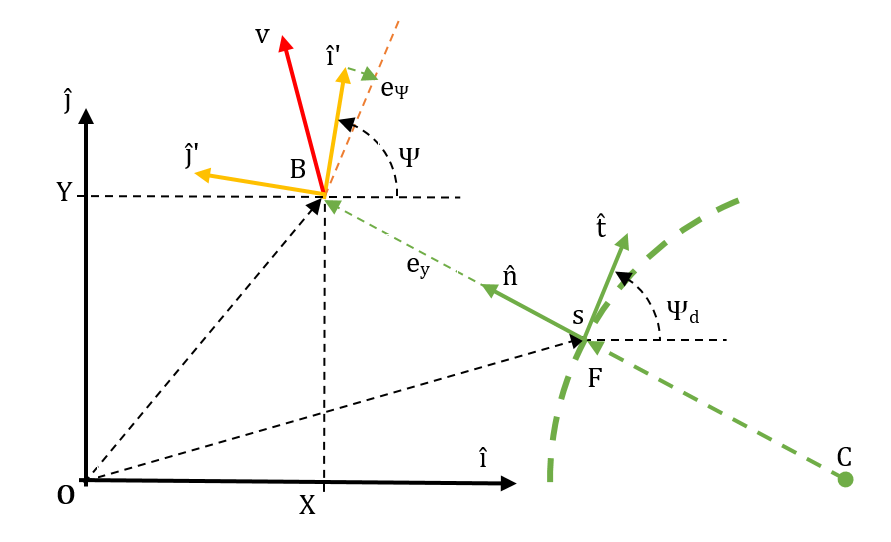
\includegraphics[width=1\linewidth]{pictures/frames}
        \caption{Global, body and track frames}
    \end{figure}
    It is considered a moving body frame B in a plane with respect to an inertial
    global frame O, and a Frenet frame F.



    \subsection{Inertial-Body transform in cartesian cordiantes}

        \subsubsection{Position transform}
            The position of a point attached to the frame body B with respect to the 
            global (inertial) frame O is given by the elementary rotation:
            \begin{equation}
                \begin{aligned}
                    & \vec{r}^O = R^O_B \vec{r}^B
                \end{aligned}
            \end{equation}
            where:
            \begin{equation}
                \begin{aligned}
                    & R^O_B = \begin{bmatrix} \cos(\psi) & -\sin(\psi)\\ \sin(\psi) & \cos(\psi) \end{bmatrix}
                \end{aligned}
            \end{equation}

        \subsubsection{Velocity transform}
            The velocity of the rotating body frame B, expressed with respect to the inertial global frame O, is:
            \begin{equation}
                \begin{aligned}
                    \vec{\dot{r}}^O & = \frac{d}{dt} (r^O) = \frac{d}{dt} \left(R^O_B \vec{r}^B\right)
                    = \frac{dR^O_B}{dt} \vec{r}^B + R^O_B \frac{d}{dt} (\vec{r}^B) = \dot{R}^O_B \vec{r}^B + R^O_B \vec{\dot{r}}^B_B \\
                    & = \vec{\omega}^O \times R^O_B \vec{r}^B + R^O_B \vec{v}^B_B = \vec{\omega}^O \times \vec{r}^O + \vec{v}^O_B \\
                \end{aligned}
            \end{equation}
            where:  $ \begin{array}[t]{l}
                        \dot{R}^O_B = \omega^O \times R^O_B \\
                        R^O_B \vec{\dot{r}}^B_B = R^O_B \vec{v}^B_B = \vec{v}^O_B \\
                    \end{array} $ \\
                \\
            then:
            \begin{equation}
                \begin{aligned}
                    \vec{v} & = \vec{v}_B + \vec{\omega} \times \vec{r} \\
                \end{aligned}
            \end{equation}

            \paragraph{Velocity decomposition}
            \begin{equation}
                \begin{aligned}
                    \vec{v} & = \vec{v}_B + \vec{\omega} \times \vec{r} \\
                    & = v_{B_x} \hat{i} + v_{B_y} \hat{j} + \omega \hat{k} \times (x \hat{i} - y \hat{j}) \\
                    & = v_{B_x} \hat{i} + v_{B_y} \hat{j} + \omega x (\hat{k} \times \hat{i}) - \omega y (\hat{k} \times \hat{j}) \\
                    & = v_{B_x} \hat{i} + v_{B_y} \hat{j} + \omega x \hat{j} + \omega y \hat{i} \\
                \end{aligned}
            \end{equation}
            then:
            \begin{equation}
                \begin{aligned}
                    & \begin{bmatrix} v_{x} \\ v_{y} \end{bmatrix}
                    = 
                    \begin{bmatrix} v_{B_x} + \omega y \\ v_{B_y} + \omega x \end{bmatrix} \\
                \end{aligned}
            \end{equation}




        \subsubsection{Acceleration transform}
            The acceleration of the rotating body frame B, expressed with respect to the inertial global frame O, is:
            \begin{equation}
                \begin{aligned}
                    \vec{\ddot{r}}^O & = \frac{d}{dt} \left(\vec{v}_B^O\right) + \frac{d}{dt} \left(\vec{\omega}^O \times \vec{r}^O\right) \\
                    & = \frac{d}{dt} \left(R^B_O \vec{v}_B^B\right) + \frac{d}{dt} \left(\vec{\omega}^O \times R^B_O \vec{r}^B\right) \\
                    & = \dot{R}^B_O \vec{v}_B^B + R^B_O \vec{\dot{v}}_B^B + \vec{\dot{\omega}}^O \times R^B_O \vec{r}^B + \vec{\omega}^O \times \dot{R}^B_O \vec{r}^B + \vec{\omega}^O \times R^B_O \vec{v}_B^B \\
                    & = \vec{\omega}^O \times \vec{v}_B^O + \vec{a}_B^O + \vec{\dot{\omega}}^O \times \vec{r}^O + \vec{\omega}^O \times (\vec{\omega}^O \times \vec{r}^O) + \vec{\omega}^O \times \vec{v}^O_B \\
                    & = \vec{a}_B^O + \vec{\omega}^O \times (\vec{\omega}^O \times \vec{r}^O) + 2 \vec{\omega}^O \times \vec{v}_B^O + \vec{\dot{\omega}}^O \times \vec{r}^O \\
                \end{aligned}
            \end{equation}
            where:  $ \begin{array}[t]{l}
                        \dot{R}^O_B = \omega^O \times R^O_B \\
                        \vec{v}_B^O = R_O^B \vec{v}_B^B \\
                        R^B_O \vec{\dot{v}}_B^B = R^B_O \vec{a}_B^B = \vec{a}_B^O
                    \end{array} $ \\
                \\
            then:
            \begin{equation}
                \begin{aligned}
                    \vec{a} & = \vec{a}_B + \vec{\omega} \times (\vec{\omega} \times \vec{r}) + 2 \vec{\omega} \times \vec{v}_B + \vec{\dot{\omega}} \times \vec{r} \\
                \end{aligned}
            \end{equation}

            \paragraph{Acceleration decomposition}
            Negletting angular accellerations and the Coriolis components, the equation can be rewritten as:
            \begin{equation}
                \begin{aligned}
                    \vec{a} & = \vec{a}_B + \vec{\omega} \times (\vec{\omega} \times \vec{r}) \\
                    & = a_{B_x} \hat{i} + a_{B_y} \hat{j} + \omega \hat{k} \times (\omega \hat{k} \times (x \hat{i} - y \hat{j})) \\
                    & = a_{B_x} \hat{i} + a_{B_y} \hat{j} + \omega^2 x (\hat{k} \times (\hat{k} \times \hat{i})) - \omega^2 y (\hat{k} \times (\hat{k} \times \hat{j})) \\
                    & = a_{B_x} \hat{i} + a_{B_y} \hat{j} - \omega^2 x \hat{i} + \omega^2 y \hat{j} \\
                    & = a_{B_x} \hat{i} + a_{B_y} \hat{j} - \omega v_{B_y} \hat{i} + \omega v_{B_x} \hat{j} \\
                \end{aligned}
            \end{equation}
            where:  $ \begin{array}[t]{l}
                        v_{B_x} = \omega y \\
                        v_{B_y} = \omega x \\
                    \end{array} $ \\
                \\
            then:
            \begin{equation}
                \label{accelleration in body frame}
                \begin{aligned}
                    & \begin{bmatrix} a_{x} \\ a_{y} \end{bmatrix}
                    = \begin{bmatrix} a_{B_x} - \omega v_{B_y} \\ a_{B_y} + \omega v_{B_u} \end{bmatrix} \\
                \end{aligned}
            \end{equation}





            \newpage


    



    \subsection{Body-Frenet transform in curvilinear coordiantes}
        The body frame B can be expressed with respect to a Frenet frame F
        on a defined track, in curvilinear cooridnates.

        \subsubsection{Position transform}
            The position of the body frame B with respect to the Frenet frame F,
            expressed in the curvilinear coordinates are:
            \begin{equation}
                \begin{aligned}
                    & s = \rho \theta \\
                    & \vec{e}_y = \vec{OB} - \vec{OF} = \vec{FB} \\
                \end{aligned}
            \end{equation}
            where the deviation from the body heading and the track curvature is:
            \begin{equation}
                \begin{aligned}
                    & e_{\psi} = \psi - \psi_d \\
                \end{aligned}
            \end{equation}
            The rotation matrix transform from the Frenet frame F to the global frame O:
            \begin{equation}
                \begin{aligned}
                    & R^F_O(\psi_d) = 
                    \begin{bmatrix} \cos{\psi_d} & -\sin{\psi_d} \\ \sin{\psi_d} & \cos{\psi_d} \end{bmatrix} \\
                \end{aligned}
            \end{equation}


        \subsubsection{Velocity transform}
            Deriving the position transorm equations:
            \begin{equation}
                \begin{aligned}
                    & \vec{\dot{s}} = \frac{d}{dt} (\rho \theta) \hat{t} = (\frac{d\rho}{dt} \theta + \rho \frac{d\theta}{dt}) \hat{t} = (\rho \frac{d\theta}{dt}) \hat{t} = \rho \omega_d \hat{t} \\
                    & \vec{\dot{e}}_y = \frac{d}{dt} (\vec{OB} - \vec{OF}) =  \frac{d}{dt} (\vec{FB}) \\
                \end{aligned}
            \end{equation}
            from which can be obtained the track angular velocity:
            \begin{equation}
                \begin{aligned}
                    & \omega_d = \frac{\dot{s}}{\rho} = \dot{s} c_c \\
                \end{aligned}
            \end{equation}
            where:  $ \begin{array}[t]{l}
                        \rho: \quad $radius of curvature$ \\
                        c_c = 1/\rho: \quad $curvature$ \\
                    \end{array} $ \\
            \\
            Referring to the picture \ref{frames}:
            \begin{equation}
                \begin{aligned}
                    & \vec{OB} = \vec{OF} + \vec{FB} \\
                \end{aligned}
            \end{equation}
            deriving with respect the time: 
            \begin{equation}
                \begin{aligned}
                    & \frac{d}{dt}(\vec{OB})^F = \frac{d}{dt}(\vec{OF})^F + \frac{d}{dt}(\vec{FB})^F + \vec{\omega}_d^O \times (\vec{FB}) \\
                    \Rightarrow & R^O_F(\psi_d) R^B_O(\psi) \frac{d}{dt}(\vec{OB})^B = \frac{d}{dt}(\vec{OF})^F + \frac{d}{dt}(\vec{FB})^F + \vec{\omega}_d^O \times (\vec{FB}) \\
                    \Rightarrow & R^O_F(\psi_d) R^B_O(\psi) \vec{v}_{OB}^B = \dot{s} \hat{t} + \dot{e}_y \hat{n} - \dot{s} e_y c_c \hat{t} \\
                \end{aligned}
            \end{equation}
            where:  $ \begin{array}[t]{l}
                        \frac{d}{dt}(\vec{OB})^F = R^O_F(\psi_d) \frac{d}{dt}(\vec{OB})^O = R^O_F(\psi_d) R^B_O(\psi) \frac{d}{dt}(\vec{OB})^B \\
                        \frac{d}{dt}(\vec{OB})^B = \vec{v}_{OB}^B \\
                        \frac{d}{dt}(\vec{OF})^F = \dot{s} \hat{t} \\
                        \frac{d}{dt}(\vec{FB})^F = \dot{e}_y \hat{n} \\
                        \vec{\omega}_d^O \times (\vec{FB}) = \dot{s} c_c \hat{k} \times e_y \hat{n} = - \dot{s} e_y c_c \hat{t} \\
                    \end{array} $ \\
            Multiplying the matrices and exploiting the trigonometric sum of angles:
            \begin{equation}
                \begin{aligned}
                    R^O_F(\psi_d) R^B_O(\psi) & =
                    \begin{bmatrix} \cos{\psi_d} & \sin{\psi_d} \\ -\sin{\psi_d} & \cos{\psi_d} \end{bmatrix} 
                    \begin{bmatrix} \cos{\psi} & -\sin{\psi} \\ \sin{\psi} & \cos{\psi} \end{bmatrix}  \\
                    & = \begin{bmatrix} \cos{(\psi-\psi_d)} & -\sin{(\psi-\psi_d)} \\ \sin{(\psi-\psi_d)} & \cos{(\psi-\psi_d)} \end{bmatrix} \\
                    & = \begin{bmatrix} \cos{e_{\psi}} & -\sin{e_{\psi}} \\ \sin{e_{\psi}} & \cos{e_{\psi}} \end{bmatrix} = R^B_F(e_{\psi}) \\
                \end{aligned}
            \end{equation}
            Replacing the matrix transform above in the previus equation:
            \begin{equation}
                \begin{aligned}
                    & R^B_F(e_{\psi}) \vec{v}_{OB}^B = \dot{s} \hat{t} + \dot{e}_y \hat{n} - \dot{s} e_y c_c \hat{t}
                    = R^B_F(e_{\psi}) \vec{v}_{OB}^B = \dot{s} (1 - e_y c_c) \hat{t} + \dot{e}_y \hat{n} \\
                \end{aligned}
            \end{equation}
            and decomposing along the Frenet frame axes:
            \begin{equation}
                \label{curvilinear dynamics}
                \begin{aligned}
                    & \begin{bmatrix} \dot{s} \\ \dot{e}_y \end{bmatrix} 
                    = 
                    R^B_F(e_{\psi}) \begin{bmatrix} v_x \\ v_y \end{bmatrix} \begin{bmatrix} \frac{1}{1 - c_c e_y} \\ 0 \end{bmatrix} \\
                \end{aligned}
            \end{equation}
            while the deviation angle velocity:
            \begin{equation}
                \label{curvilinear deviation}
                \begin{aligned}
                    & \vec{\dot{e}}_{\psi} = \frac{d}{dt} (\psi - \psi_d) \hat{k} = \vec{\omega} - \vec{\omega}_d = \vec{\omega} - \vec{\dot{s}} c_c \\
                \end{aligned}
            \end{equation}







        \newpage





    \subsection{Inertial-Frenet-Body transfrom}

        \subsubsection{Rotation matrix}
            Rotation matrix between the inertial/global frame O, body frame B and Frenet frame F:
            \begin{equation}
                \begin{aligned}
                    & R_B^O(\psi) = \begin{bmatrix} \cos{\psi} & -\sin{\psi} \\ \sin{\psi} & \cos{\psi} \end{bmatrix}  \\
                    & R_F^O(\psi_d) = \begin{bmatrix} \cos{\psi_d} & -\sin{\psi_d} \\ \sin{\psi_d} & \cos{\psi_d} \end{bmatrix} \\
                    & R_B^F(e_{\psi}) = \begin{bmatrix} \cos{e_{\psi}} & -\sin{e_{\psi}} \\ \sin{e_{\psi}} & \cos{e_{\psi}} \end{bmatrix} \\
                \end{aligned}
            \end{equation}


        \subsubsection{Coordinate system transform}
            \begin{equation}
                \begin{aligned}
                    & s = \vec{r}_{OF}^F \\
                    & \vec{e}_y = \vec{r}_{FB}^F \\
                    & e_{\psi} = \psi - \psi_d \\
                \end{aligned}
            \end{equation}
            The curvilinear abscissa $s$ can be expressed in polar coordinates
            \begin{equation}
                \begin{aligned}
                    & s = \rho \theta \\
                \end{aligned}
            \end{equation}
            where:  $ \begin{array}[t]{l}
                \rho: \quad $curve radius$ \\
                c_c = 1/\rho: \quad $curvature$ \\
                \theta: \quad $angle travelled$ \\
            \end{array} $ \\
            which can be derived with respect to the time, considering a constant curvature:
            \begin{equation}
                \begin{aligned}
                    & \vec{\dot{s}} = \frac{d}{dt}(\rho \theta) \hat{t} = \rho \frac{d}{dt}(\theta) \hat{t} = \rho \omega_d \hat{t} \\
                \end{aligned}
            \end{equation}
            then the angular velocity:
            \begin{equation}
                \begin{aligned}
                    & \omega_d = \frac{\dot{s}}{\rho} = \dot{s} c_c \\
                \end{aligned}
            \end{equation}



            
        \subsubsection{Position}
            \begin{equation}
                \begin{aligned}
                    & \vec{r}_{OB}^O = \vec{r}_{OF}^O + \vec{r}_{FB}^O = \vec{r}_{OF}^O + R_F^O(\psi_d) \vec{r}_{FB}^F
                \end{aligned}
            \end{equation}


        \subsubsection{Velocity}
            \begin{equation}
                \begin{aligned}
                    & \vec{v}_B^O = R_B^O(\psi) \vec{v}_B^B \\
                    & \vec{v}_B^F = R_B^F(e_{\psi}) \vec{v}_B^B \\
                \end{aligned}
            \end{equation}
            Deriving the position vector $\vec{r}_{OB}^O$ with respect the time: 
            \begin{equation}
                \begin{aligned}
                    & \frac{d}{dt}(\vec{r}_{OB}^O) = \frac{d}{dt}(\vec{r}_{OF}^O) + \frac{d}{dt}(R_F^O(\psi_d) \vec{r}_{FB}^F) \\
                    \Rightarrow & \vec{v}_B^O = \frac{d}{dt}(\vec{r}_{OF}^O) + \dot{R}_F^O(\psi_d) \vec{r}_{FB}^F + R_F^O(\psi_d) \vec{\dot{r}}_{FB}^F \\
                    \Rightarrow & \vec{v}_B^O = \vec{\dot{r}}_{OF}^O + \vec{\omega}_F^O \times R_F^O(\psi_d) \vec{r}_{FB}^F + R_F^O(\psi_d) \vec{\dot{r}}_{FB}^F \\
                    \Rightarrow & R_O^F(\psi_d) \vec{v}_B^O = R_O^F(\psi_d) \vec{\dot{r}}_{OF}^O + \vec{\omega}_F^O \times \vec{r}_{FB}^F + \vec{\dot{r}}_{FB}^F \\
                    \Rightarrow & R_O^F(\psi_d) R_B^O(\psi) \vec{v}_B^B = \vec{\dot{r}}_{OF}^F + \vec{\omega}_F^O \times \vec{r}_{FB}^F + \vec{\dot{r}}_{FB}^F \\
                    \Rightarrow & R_F^BF(e_{\psi}) \vec{v}_B^B = \vec{\dot{r}}_{OF}^F + \vec{\omega}_F^O \times \vec{r}_{FB}^F + \vec{\dot{r}}_{FB}^F \\
                \end{aligned}
            \end{equation}
            where:  $ \begin{array}[t]{l}
                        R_F^BF(e_{\psi}) = R_O^F(\psi_d) R_B^O(\psi)
                    \end{array} $ \\
                    \\
            Passing from the cartesian coordinates to the curvilinear coordinates:
            \begin{equation}
                \begin{aligned}
                    & R_F^B(e_{\psi}) \vec{v}_B^B = \vec{\dot{s}} + \vec{\omega}_d \times \vec{e}_y + \vec{\dot{e}}_y \\
                    \Rightarrow & R_F^B(e_{\psi}) \vec{v}_B^B = \dot{s} \hat{t} + \dot{s} c_c \hat{k} \times e_y \hat{n} + \dot{e}_y \hat{n} \\
                    \Rightarrow & R_F^B(e_{\psi}) \vec{v}_B^B = \dot{s} \hat{t} + \dot{s} e_y c_c (-\hat{t}) + \dot{e}_y \hat{n} \\
                    \Rightarrow & R_F^B(e_{\psi}) \vec{v}_B^B = \dot{s} (1 - e_y c_c ) \hat{t} + \dot{e}_y \hat{n} \\
                \end{aligned}
            \end{equation}
            which can be decompoed in the Frenet frame axes:
            \begin{equation}
                \begin{aligned}
                    & \begin{bmatrix} \dot{s} \\ \dot{e}_y \end{bmatrix} 
                    = 
                    R^B_F(e_{\psi}) \begin{bmatrix} v_x \\ v_y \end{bmatrix} \begin{bmatrix} \frac{1}{1 - c_c e_y} \\ 0 \end{bmatrix} \\
                \end{aligned}
            \end{equation}
            while the deviation angle velocity:
            \begin{equation}
                \begin{aligned}
                    & \vec{\dot{e}}_{\psi} = \frac{d}{dt} (\psi - \psi_d) \hat{k} = \vec{\omega} - \vec{\omega}_d = \vec{\omega} - \dot{s} c_c \hat{k} \\
                \end{aligned}
            \end{equation}




    \newpage




%============================================================================
% SECTION 2
%============================================================================



\section{Bicycle dynamic model}
    Ref: \cite{Vehicle dynamics ancd control} (pg. 27), \cite{MPC for Autonomous Vehicles} \\
    \begin{figure}[h]
        \centering
        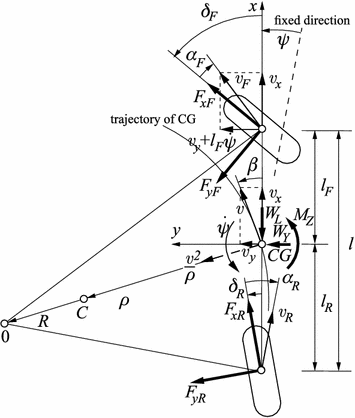
\includegraphics[width=0.5\linewidth]{pictures/bicycle_model}
        \caption{Bicycle dynamics}
    \end{figure} \\
    From equations \ref{accelleration in body frame}, changing the notation as follow:
    \begin{equation}
        \begin{aligned}
            & \begin{bmatrix} a_{x} \\ a_{y} \end{bmatrix}
            = \begin{bmatrix} a_{B_x} - \omega v_{B_x} \\ a_{B_y} + \omega v_{B_y} \end{bmatrix} 
            \longrightarrow 
            \begin{bmatrix} a_{x}^O \\ a_{y}^O \end{bmatrix}
            = \begin{bmatrix} \dot{v}_x - \omega_z v_y \\ \dot{v}_y + \omega_z v_x \end{bmatrix} \\
        \end{aligned}
    \end{equation}
    it is possible to write the dynamic equation for a bicycle:
    \begin{equation}
        \label{bicycle dynamics I}
        \begin{aligned}
            & m a_{x}^O = m (\dot{v}_x - \omega_z v_y) = F_{xf} + F_{xr} \\
            & m a_{y}^O = m (\dot{v}_y + \omega_z v_x) = F_{yf} + F_{yr} \\
            & I_z \dot{\omega}_z = l_f F_{yf} - l_r F_{yr} \\
        \end{aligned}
    \end{equation}
    where:  $ \begin{array}[t]{l}
                m: \quad $mass$ \\
                l_f, l_r: \quad $front and rear wheel distance from the center of mass $ \\
                F_{xf}, F_{xr}: \quad $Forces on x body axis of front (f) and rear (r) wheel$ \\
                F_{yf}, F_{yr}: \quad $Forces on y body axis of front (f) and rear (r) wheel$ \\
            \end{array} $ \\
    in which the forces can be decomposed in the tire-fixed frame:
    \begin{equation}
    \label{wheel forces I}
    \begin{cases}
        F_{x,i} = F_{l,i} cos(\delta_i) - F_{s,i} sin(\delta_i) \\
        F_{y,i} = F_{l,i} sin(\delta_i) + F_{s,i} cos(\delta_i) \\
    \end{cases}
    \end{equation}
    where:  $ \begin{array}[t]{l}
                F_{l,i} = \{F_{lf}, F_{lr}\}: \quad $Force on longitudinal axis of front (f) and rear (r) wheel$ \\
                F_{s,i} = \{F_{sf}, F_{sr}\}: \quad $Force on perpendicular axis of front (f) and rear (r) wheel$ \\
                \delta_i = \{delta_f, delta_r\}: \quad $Front (f) and rear (r) wheel steering angles$ \\
            \end{array} $ \\
    \\
    Replacing the equations \ref{wheel forces I} into \ref{bicycle dynamics I}, it is obtained the complete formulation:
    \begin{equation}
        \label{bicycle dynamics II}
        \begin{aligned}
            \dot{v}_x = \frac{1}{m} (F_{lf} \cos(\delta_f) - F_{sf} \sin(\delta_f) + F_{lr} \cos(\delta_r) - F_{sr} \sin(\delta_r)) + \omega_z v_y  \\
            \dot{v}_y = \frac{1}{m} (F_{lf} \sin(\delta_f) + F_{sf} \cos(\delta_f) + F_{lr} \sin(\delta_r) + F_{sr} \cos(\delta_r)) - \omega_z v_x  \\
            \dot{\omega}_z = \frac{1}{I_z} (l_f(F_{lf} \sin(\delta_f) + F_{sf} \cos(\delta_f)) - l_r(F_{lr} \sin(\delta_r) + F_{sr} \cos(\delta_r))) \\
        \end{aligned}
    \end{equation}






    
    \paragraph{Sideslip angle}
        Ref: \cite{Vehicle dynamics ancd control} (pg. 27) \\
        \begin{figure}[h]
            \centering
            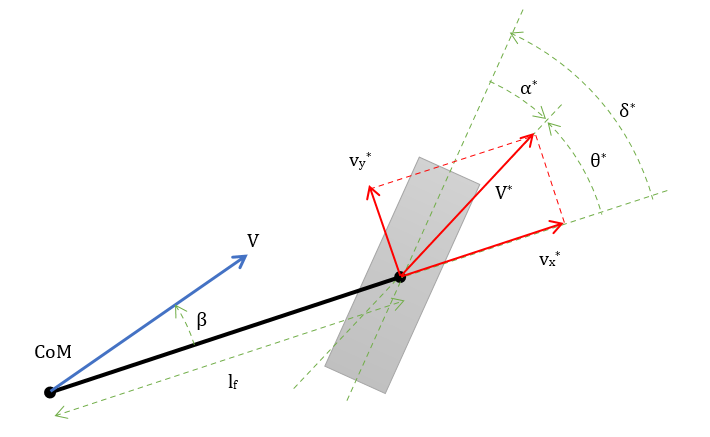
\includegraphics[width=0.75\linewidth]{pictures/sideslip_angle}
            \caption{Sideslip angle}
        \end{figure} \\
        The sideslip angle is defined as:
        \begin{equation}
            \begin{aligned}
                & \alpha_{*} = \delta_{*} - \theta_{*} \\
            \end{aligned}
        \end{equation}
        where:  $ \begin{array}[t]{l}
                    \theta_{*} = \arctan\left(\frac{v_{x*}}{v_{y*}}\right) \\
                    v_{x*}, v_{y*}: \quad $longitudinal and lateral wheel velocities in fixed body-frame$ \\
                \end{array} $ \\
        While $v_{x*}$ coincides with the CoM longitudinal velocity, the $v_{y*}$
        is the sum of the CoM lateral velocity and the tangential velocity of the wheel
        respect to the CoM due to the angular velocity, then:
        \begin{equation}
            \begin{aligned}
                & v_{xf} = v_{xr} = v_{x} \\
                & v_{yf} = v_{y} + l_f \omega_z \\
                & v_{yr} = v_{y} - l_r \omega_z \\
            \end{aligned}
        \end{equation}
        where:  $ \begin{array}[t]{l}
                    v_{xf}, v_{yf}: \quad $front wheel velocities in fixed body-frame$ \\
                    v_{xr}, v_{yr}: \quad $rear wheel velocities in fixed body-frame$ \\
                \end{array} $ \\
        Replacing the equation above in the first one, it is obtained the sideslip angle
        of the front and the rear wheel:
        \begin{equation}
            \label{sideslip angle equation}
            \begin{aligned}
                & \alpha_f = \delta_f - \arctan \left(\frac{v_y + l_f \omega_z}{v_x}\right)   \\ 
                & \alpha_r = \delta_r - \arctan \left(\frac{v_y - l_r \omega_z}{v_x}\right)   \\  
            \end{aligned}
        \end{equation}




    \subsection{Tire's linear dynamic}
        Ref: \cite{MPC for Autonomous Vehicles} \\
        For small sideslip angles, the wheel lateral force can be well approximated 
        proportional to the sideslip angle itself:
        \begin{equation}
            \begin{aligned}
                & F_{sf} = C_f(F_z, \mu) \alpha_f  \\
                & F_{sr} = C_r(F_z, \mu) \alpha_r  \\
            \end{aligned}
        \end{equation}
        where $C_f, C_r$ is the "Cornering stiffness" of each wheel, depending on the
        normal force acting on the wheel and the friction coefficient with the surface. \\
        Here, an estimate of this coefficient has been done evaluating the dynamic evolution
        of the nonlinear plant model, with different values of the cornering stiffness,
        until a realistic behaviour has been achieved. \\
        To notice is that small values of the cornering stiffness, make difficult the
        steering, while too high values generate excessively high lateral forces also
        for small sideslip angles, which are incompatible with the reality. \\




        \newpage

%============================================================================
% SECTION 3
%============================================================================

\section{Bicycle dynamics in a curvilinear reference for MPC prediction}
    From the previous sections, a dynamic model of the bicycle in a 
    curvilinear reference can be implemented under the following assumptions:
    \begin{itemize}
        \item Small sideslip angles ($\alpha \leq 10° \rightarrow \sin(\Delta) \simeq \Delta, \cos(\Delta) \simeq 1 $)
        \item Front steering wheel command ($\delta_r = 0$)
        \item Rear traction ($F_{lr} = T, F_{lf} = 0$)
        \item The forces are multiplied by a factor of 2 in order to take into account
        the physics of 4 wheels
    \end{itemize}
    the dynamics in \ref{bicycle dynamics II} can be semplified as:
    \begin{equation}
        \label{bicycle semplified dynamics}
        \begin{aligned}
            & \dot{v}_x = \frac{1}{m} (- F_{sf} \sin(\delta_f) + T) + \omega_z v_y  \\
            & \dot{v}_y = \frac{1}{m} (F_{sf} \cos(\delta_f) + F_{sr}) - \omega_z v_x  \\
            & \dot{\omega}_z = \frac{1}{I_z} (l_f F_{sf} \cos(\delta_f) - l_r F_{sr}) \\
        \end{aligned}
    \end{equation}
    while the sideslip angle, from \ref{sideslip angle equation}, under the assumption of
    small angles, is:
    \begin{equation}
        \begin{aligned}
            & \alpha_f = \delta_f - \arctan \left(\frac{v_y + l_f \omega_z}{v_x}\right) \simeq \delta_f - \frac{v_y + l_f \omega_z}{v_x}   \\ 
            & \alpha_r = - \arctan \left(\frac{v_y - l_r \omega_z}{v_x}\right) \simeq - \frac{v_y - l_r \omega_z}{v_x}  \\  
        \end{aligned}
    \end{equation}
    \\
    The tire's forces are then:
    \begin{equation}
        \label{linear tire semplified dynamics}
        \begin{aligned}
            & F_{sf} = 2 C_f \alpha_f \simeq 2 C_f \left(\delta_f - \frac{v_y + l_f \omega_z}{v_x} \right)  \\
            & F_{sr} = 2 C_r \alpha_r \simeq 2 C_r \left(- \frac{v_y - l_r \omega_z}{v_x}\right)  \\
        \end{aligned}
    \end{equation}
    While the link between the dynamics from the cartesian coordinate into the
    curvilinear cooridnate from \ref{curvilinear dynamics} is:
    \begin{equation}
        \label{curvilinear dynamics II}
        \begin{aligned}
            & \dot{s}(t) = \frac{v_x \cos{e_{\psi}} - v_y \sin{e_{\psi}}}{1 - c_c(s) e_y}   \\
            & \dot{e}_y(t) = v_x \sin{e_{\psi}} + v_y \cos{e_{\psi}}  \\
            & \dot{e}_{\psi}(t) = \omega_z - \frac{v_x \cos{e_{\psi}} - v_y \sin{e_{\psi}}}{1 - c_c(s) e_y} c_c(s)  \\
        \end{aligned}
    \end{equation}
    \\
    Putting toghether \ref{bicycle semplified dynamics} \ref{linear tire semplified dynamics} \ref{curvilinear dynamics II}
    it is obtained the complete dynamics:
    \begin{equation}
        \begin{aligned}
            & \dot{v}_x = a + \frac{2}{m} \left(- C_f \left(\delta_f - \frac{v_y + l_f \omega_z}{v_x}\right) \sin(\delta_f)\right)  + v_y \omega_z   \\
            & \dot{v}_y = \frac{2}{m} \left(C_f \left(\delta_f - \frac{v_y + l_f \omega_z}{v_x}\right) \cos(\delta_f) + C_r \left(- \frac{v_y - l_r \omega_z}{v_x}\right)\right)  - v_x \omega_z   \\
            & \dot{\omega}_z = \frac{2}{I_z} \left(l_f C_f \left(\delta_f - \frac{v_y + l_f \omega_z}{v_x}\right) \cos(\delta_f) - l_r C_r \left(- \frac{v_y - l_r \omega_z}{v_x}\right)\right)  \\
            & \dot{s}(t) = \frac{v_x \cos{e_{\psi}} - v_y \sin{e_{\psi}}}{1 - c_c(s) e_y}   \\
            & \dot{e}_y(t) = v_x \sin{e_{\psi}} + v_y \cos{e_{\psi}}  \\
            & \dot{e}_{\psi}(t) = \omega_z - \frac{v_x \cos{e_{\psi}} - v_y \sin{e_{\psi}}}{1 - c_c(s) e_y} c_c(s)  \\
        \end{aligned}
    \end{equation}
    where:  $ \begin{array}[t]{l}
                \xi = \begin{bmatrix} v_x & v_y & \omega_z & s & e_y & e_{\psi} \end{bmatrix}^T \\
                u = \begin{bmatrix} \delta_f & a \end{bmatrix}^T \\
            \end{array} $ \\



            \newpage



%============================================================================
% SECTION 4
%============================================================================

\section{MPC}


    \subsection{Model linearization}
        The nonlinear system has to be linearized around the 
        operative point $p = [\xi_0, u_0]$.
        The system can be approximated through the Taylor expansion, stopped
        to the first derivative:
        \begin{equation}
            \begin{aligned}
                \frac{d}{dt}(\Delta \xi(t)) \approx \frac{\partial f}{\partial \xi} \Delta \xi(t) + \frac{\partial f}{\partial u} \Delta u(t)
                & \Rightarrow 
                \Delta \dot{\xi}(t) \approx A(p) \Delta \xi(t) + B(p) \Delta u(t) \\
            \end{aligned}
        \end{equation}
        Changing the notation for semplicity, the new state/input definition is defined 
        as the state error with respect the operative point:
        \begin{equation}
            \begin{aligned}
                & \dot{\xi}(t) = A(p) \xi(t) + B(p) u(t) \\
            \end{aligned}
        \end{equation}
        where:  $ \begin{array}[t]{l}
                    \xi = \begin{bmatrix} \Delta v_{x0} & \Delta v_{y0} & \omega_{z0} & \Delta s_0 & \Delta e_{y0} & \Delta e_{\psi 0} \end{bmatrix}^T \\
                    u = \begin{bmatrix} \Delta \delta_{f0} & \Delta a_0 \end{bmatrix}^T \\               
                    A(p) = \frac{\partial f}{\partial \xi} \\
                    B(p) = \frac{\partial f}{\partial u}   \\   
                \end{array} $ \\


        \paragraph{Linearized QP matrices}
        \begin{equation}
            \begin{aligned}
                & A = J_f(x) 
                = 
                \begin{bmatrix} 
                    A_{11} & A_{12} \\
                    A_{21} & A_{22} \\
                \end{bmatrix}
                =
                \begin{bmatrix} 
                    \frac{\partial \dot{v}_x}{\partial v_x} & \frac{\partial \dot{v}_x}{\partial v_y} & \frac{\partial \dot{v}_x}{\partial \omega_z} & \frac{\partial \dot{v}_x}{\partial s} & \frac{\partial \dot{v}_x}{\partial e_y} &  \frac{\partial \dot{v}_x}{\partial e_{\psi}} \\
                    \frac{\partial \dot{v}_y}{\partial v_x} & \frac{\partial \dot{v}_y}{\partial v_y} & \frac{\partial \dot{v}_y}{\partial \omega_z} & \frac{\partial \dot{v}_y}{\partial s} & \frac{\partial \dot{v}_y}{\partial e_y} & \frac{\partial \dot{v}_y}{\partial e_{\psi}}\\
                    \frac{\partial \dot{\omega}_z}{\partial v_x} & \frac{\partial \dot{\omega}_z}{\partial v_y} & \frac{\partial \dot{\omega}_z}{\partial \omega_z} & \frac{\partial \dot{\omega}_z}{\partial s} & \frac{\partial \dot{\omega}_z}{\partial e_y} & \frac{\partial \dot{\omega}_z}{\partial e_{\psi}} \\
                    \frac{\partial \dot{s}}{\partial v_x} & \frac{\partial \dot{s}}{\partial v_y} & \frac{\partial \dot{s}}{\partial \omega_z} & \frac{\partial \dot{s}}{\partial s} & \frac{\partial \dot{s}}{\partial e_y} & \frac{\partial \dot{s}}{\partial e_{\psi}} \\ 
                    \frac{\partial \dot{e}_y}{\partial v_x} & \frac{\partial \dot{e}_y}{\partial v_y} & \frac{\partial \dot{e}_y}{\partial \omega_z} & \frac{\partial \dot{e}_y}{\partial s} & \frac{\partial \dot{e}_y}{\partial e_y} & \frac{\partial \dot{e}_y}{\partial e_{\psi}} \\ 
                    \frac{\partial \dot{e}_{\psi}}{\partial v_x} & \frac{\partial \dot{e}_{\psi}}{\partial v_y} & \frac{\partial \dot{e}_{\psi}}{\partial \omega_z} & \frac{\partial \dot{e}_{\psi}}{\partial s} & \frac{\partial \dot{e}_{\psi}}{\partial e_y} & \frac{\partial \dot{e}_{\psi}}{\partial e_{\psi}} \\ 
                \end{bmatrix}
            \end{aligned}
        \end{equation}

        
        % $A_{11}$ \\
        $\begin{aligned}
            & \frac{\partial \dot{v}_x}{\partial v_x} = \frac{2 C_f \sin(\delta_{f0}) (v_{y0} + l_f \omega_{z0})}{m v_{x0}^2} \\
            & \frac{\partial \dot{v}_x}{\partial v_y} = \frac{2 C_f \sin(\delta_{f0})}{m v_{x0}} + \omega_{z0} \\
            & \frac{\partial \dot{v}_x}{\partial \omega_z} = \frac{2 C_f l_f \sin(\delta_{f0})}{m v_{x0}} + v_{y0} \\
        \end{aligned}$

        $\begin{aligned}
            & \frac{\partial \dot{v}_y}{\partial v_x} = -\frac{2}{m v_{x0}^2} \left[ C_f (v_{y0} + l_f \omega_{z0}) \cos(\delta_{f0}) + C_r (v_{y0} - l_r \omega_{z0}) \right] - \omega_{z0} \\
            & \frac{\partial \dot{v}_y}{\partial v_y} = -\frac{2}{m v_{x0}} \left[ C_f \cos(\delta_{f0}) + C_r \right]   \\
            & \frac{\partial \dot{v}_y}{\partial \omega_z} = -\frac{2}{m v_{x0}} \left[ C_f l_f \cos(\delta_{f0}) - C_r l_r \right]  - v_{x0} \\ 
        \end{aligned}$

        $\begin{aligned}
            & \frac{\partial \dot{\omega}_z}{\partial v_x} = \frac{2}{I_z v_{x0}^2} \left[ C_f l_f(v_{y0} + l_f \omega_{z0})\cos(\delta_{f0}) - C_r l_r(v_{y0} - l_r \omega_{z0}) \right]  \\ % \frac{C_f l_f \sin(\delta_{f0}) (v_{y0} + l_f \omega_{z0}) + C_r l_r (-v_{y0} + l_r \omega_{z0})}{I_z v_{x0}^2}\\
            & \frac{\partial \dot{\omega}_z}{\partial v_y} = \frac{2}{I_z v_{x0}} \left[ - C_f l_f \cos(\delta_{f0}) + C_r l_r \right]  \\ % \frac{- C_f l_f \sin(\delta_{f0}) + C_r l_r}{I_z v_{x0}} \\
            & \frac{\partial \dot{\omega}_z}{\partial \omega_z} = \frac{2}{I_z v_{x0}} \left[ - C_f l_f^2 \cos(\delta_{f0}) - C_r l_r^2 \right]  \\ % \frac{- C_f l_f^2 \sin(\delta_{f0}) - C_r l_r^2}{I_z v_{x0}} \\
        \end{aligned}$

            
        % $A_{22}$
        $\begin{aligned}
            & \frac{\partial \dot{s}}{\partial s} = 0 \\
            & \frac{\partial \dot{s}}{\partial e_y} = \frac{v_{x0} \cos(e_{\psi 0})-v_{y0} \sin(e_{\psi 0})}{(1 - c_c e_{y0})^2} c_c \\
            & \frac{\partial \dot{s}}{\partial e_{\psi}} = \frac{-v_{x0} \sin(e_{\psi 0})-v_{y0} \cos(e_{\psi 0})}{(1 - c_c e_{y0})^2} c_c \\
        \end{aligned}$

        $\begin{aligned}
            & \frac{\partial \dot{e}_y}{\partial s} = 0 \\
            & \frac{\partial \dot{e}_y}{\partial e_y} = 0 \\
            & \frac{\partial \dot{e}_y}{\partial e_{\psi}} = v_{x0} \cos(e_{\psi 0}) - v_{y0} \sin(e_{\psi 0}) \\
        \end{aligned}$

        $\begin{aligned}
            & \frac{\partial \dot{e}_{\psi}}{\partial s} = 0 \\
            & \frac{\partial \dot{e}_{\psi}}{\partial e_y} = \frac{- v_{x0} \cos(e_{\psi 0}) - v_{y0} \sin(e_{\psi 0})}{(1 - c_c e_{y0})^2} c_c^2 \\
            & \frac{\partial \dot{e}_{\psi}}{\partial e_{\psi}} = \frac{v_{x0} \sin(e_{\psi 0}) + v_{y0} \cos(e_{\psi 0})}{(1 - c_c e_{y0})} c_c \\
        \end{aligned}$


        % $A_{12}$
        $\begin{aligned}
            & \frac{\partial \dot{v}_x}{\partial s} = \frac{\partial \dot{v}_x}{\partial e_y} = \frac{\partial \dot{v}_x}{\partial e_{\psi}} = 0 \\
            & \frac{\partial \dot{v}_y}{\partial s} = \frac{\partial \dot{v}_y}{\partial e_y} = \frac{\partial \dot{v}_y}{\partial e_{\psi}} = 0 \\
            & \frac{\partial \dot{\omega}_z}{\partial s} = \frac{\partial \dot{\omega}_z}{\partial e_y} = \frac{\partial \dot{\omega}_z}{\partial e_{\psi}} = 0 \\
        \end{aligned}$


        % $A_{21}$
        $\begin{aligned}
            & \frac{\partial \dot{s}}{\partial v_x} = \frac{\cos(e_{\psi 0})}{1 - c_c e_{y0}} \\ 
            & \frac{\partial \dot{s}}{\partial v_y} = - \frac{\sin(e_{\psi 0})}{1 - c_c e_{y0}} \\ 
            & \frac{\partial \dot{s}}{\partial \omega_z} = 0 \\
        \end{aligned}$

        $\begin{aligned}
            & \frac{\partial \dot{e_y}}{\partial v_x} = \sin(e_{\psi 0}) \\ 
            & \frac{\partial \dot{e_y}}{\partial v_y} = \cos(e_{\psi 0}) \\ 
            & \frac{\partial \dot{e_y}}{\partial \omega_z} = 0 \\
        \end{aligned}$

        $\begin{aligned}
            & \frac{\partial \dot{e_{\psi}}}{\partial v_x} = - \frac{\cos(e_{\psi 0})}{1 - c_c e_{y0}} c_c \\
            & \frac{\partial \dot{\psi}}{\partial v_y} = \frac{\sin(e_{\psi 0})}{1 - c_c e_{y0}} c_c \\
            & \frac{\partial \dot{e_{\psi}}}{\partial \omega_z} = 1 \\
        \end{aligned}$



        \begin{equation}
            \begin{aligned}
                & B = J_f(u)
                = 
                \begin{bmatrix} 
                    B_{1} \\
                    B_{2} \\
                \end{bmatrix}
                =
                \begin{bmatrix} 
                    \frac{\partial \dot{v}_x}{\partial \delta_f} & \frac{\partial \dot{v}_x}{\partial a}   \\
                    \frac{\partial \dot{v}_y}{\partial \delta_f} & \frac{\partial \dot{v}_y}{\partial a}   \\
                    \frac{\partial \dot{\omega}_z}{\partial \delta_f} & \frac{\partial \dot{\omega}_z}{\partial a}   \\
                    \frac{\partial \dot{s}}{\partial \delta_f} & \frac{\partial \dot{s}}{\partial a}   \\
                    \frac{\partial \dot{e_y}}{\partial \delta_f} & \frac{\partial \dot{e_y}}{\partial a}   \\
                    \frac{\partial \dot{e_{\psi}}}{\partial \delta_f} & \frac{\partial \dot{\psi}}{\partial a}   \\
                \end{bmatrix}  \\
            \end{aligned}
        \end{equation}



        % $B_{1}$
        $\begin{aligned}
            & \frac{\partial \dot{v}_x}{\partial \delta_f} = -\frac{2 C_f}{m} \left[ \sin(\delta_{f0}) + \left( \delta_{f0} - \frac{v_{y0}+l_f}{v_{x0}} \right) \cos(\delta_{f0})  \right]   \\
            & \frac{\partial \dot{v}_x}{\partial a} = 1 \\
            & \frac{\partial \dot{v}_y}{\partial \delta_f} = \frac{2 C_f}{m} \left[ \left( - \delta_{f0} + \frac{v_{y0}+l_f w_{z0}}{v_{x0}} \right) \sin(\delta_{f0}) + \cos(\delta_{f0}) \right] \\
            & \frac{\partial \dot{v}_y}{\partial a} = 0 \\
            & \frac{\partial \dot{\omega}_z}{\partial \delta_f} = \frac{2 C_f l_f}{m} \left[ \left( - \delta_{f0} + \frac{v_{y0}+l_f w_{z0}}{v_{x0}} \right) \sin(\delta_{f0}) + \cos(\delta_{f0}) \right] \\
            & \frac{\partial \dot{\omega}_z}{\partial a} = 0 \\
        \end{aligned}$


        % $B_{2}$
        $\begin{aligned}
            & \frac{\partial \dot{s}}{\partial \delta_f} = \frac{\partial \dot{s}}{\partial a} = 0 \\
            & \frac{\partial \dot{e_y}}{\partial \delta_f} = \frac{\partial \dot{e_y}}{\partial a} = 0 \\
            & \frac{\partial \dot{e_{\psi}}}{\partial \delta_f} = \frac{\partial \dot{e_{\psi}}}{\partial a} = 0 \\
        \end{aligned}$





    \subsection{Discretization}
        The system model is discretized according the Euler approximation:
        \begin{equation}
            A_d = I + A T_s \\
            B_d = A*T_s \\
        \end{equation}
        where:  $ \begin{array}[t]{l}
                    Ts: \quad $MPC sampling time$
                \end{array} $ \\


    \subsection{Prediction}
        At k-th sampled, the predicted state is:
        \begin{equation}
            \xi_{i+1|k} = A_d(p) \xi_{i|k} + B_d(p) u_{i|k}, \quad \xi_{0|k} = \xi_{k}
        \end{equation}
        \\
        State prediction:
        \begin{equation}
            \bar{\xi}_{k} = \bar{A}_d(p) \xi_k + \bar{B}_d(p) U_k
        \end{equation}
        where:  $ \begin{array}[t]{l}
                    \bar{\xi}_{k} = \begin{bmatrix} \xi_{1|k} \\ \vdots \\ \xi_{N_p|k}  \end{bmatrix} \in \mathbb{R}^{n_x N_p}; \quad
                    U_k = \begin{bmatrix} u_{0|k} \\ \vdots \\ u_{N_c-1|k}  \end{bmatrix} \in \mathbb{R}^{n_u N_c};
                    \\
                    \bar{A}_d(p) = \begin{bmatrix} A_d(p) \\ A_d^2(p) \\ \vdots \\ A_d^{N_p}(p)  \end{bmatrix} \in \mathbb{R}^{n_x N_p,n_x}; \\
                    \bar{B}_d(p) = \begin{bmatrix} 
                                    B_d(p) & 0^{n_x,n_u} & \cdots & 0^{n_x,n_u} \\ 
                                    A_d(p) B_d(p) & B_d(p) & \cdots & 0^{n_x,n_u} \\ 
                                    \vdots & \vdots & \ddots & \vdots \\ 
                                    A_d^{N_c}(p) B_d(p) & A_d^{N_c-1}(p) B_d(p) & \cdots & B_d(p) \\ 
                                    \vdots & \vdots & \ddots & \vdots \\ 
                                    A_d^{N_p-1}(p) B_d(p) & A_d^{N_p-2}(p) B_d(p) & \cdots & A_d^{N_p-N_c}(p) B_d(p) \\ 
                                \end{bmatrix} \in \mathbb{R}^{n_x N_p,n_u N_c} \\
                \end{array} $ \\






                
                
    \subsection{Optimization}


        \subsubsection{Objective function}
            \begin{equation}
                \begin{aligned}
                    J(\xi_k)    & = \sum_{i = 1}^{N_p} \left\lVert \xi_{i|k} - ref_{i|k} \right\rVert^{2}_{Q} + \sum_{i = 0}^{N_c-1} \left\lVert u_{i|k} \right\rVert^{2}_{R} \\
                                & = \left\lVert \bar{\xi}_{k} - ref_{k} \right\rVert^{2}_{\bar{Q}} + \left\lVert U_{k} \right\rVert^{2}_{\bar{R}} \\
                                & = U_k^T \left( \bar{R} + \bar{B}_d^T \bar{Q} \bar{B}_d \right) U_k 
                                    + 2 \left( \bar{A}_d \xi_{k} - ref_{k} \right)^T \bar{Q} \bar{B}_d U_k \\
                                & + \left( \bar{A}_d \xi_{k} - ref_{k} \right)^T \bar{Q} \left( \bar{A}_d \xi_k - ref_{k} \right) \\
                \end{aligned}
            \end{equation}
            where:  $ \begin{array}[t]{l}
                        ref_{k} =   \begin{bmatrix} ref_{1|k} & \cdots & ref_{N_p|k} \end{bmatrix}^T
                        \in \mathbb{R}^{n_x N_p}
                        \\
                        \bar{Q} =  \begin{bmatrix}  
                                        Q & 0 & \cdots & 0 \\ 
                                        0 & Q & \cdots & 0 \\ 
                                        \vdots & \vdots & \ddots & \vdots \\ 
                                        0 & 0 & \cdots & Q \\ 
                                    \end{bmatrix} 
                        \in \mathbb{R}^{n_x N_p,n_x N_p}
                        \\
                        \bar{R} =  \begin{bmatrix}  
                                        \bar{\bar{R}} & 0 & \cdots & 0 \\ 
                                        0 & 0 & \cdots & 0 \\ 
                                        \vdots & \vdots & \ddots & \vdots \\ 
                                        0 & 0 & \cdots & 0 \\ 
                                    \end{bmatrix}
                        \in \mathbb{R}^{n_u N_p,n_u N_p};\
                        
                        \bar{\bar{R}} = \begin{bmatrix}  
                                            R & 0 & \cdots & 0 \\ 
                                            0 & R & \cdots & 0 \\ 
                                            \vdots & \vdots & \ddots & \vdots \\ 
                                            0 & 0 & \cdots & R \\ 
                                        \end{bmatrix}
                        \in \mathbb{R}^{n_u N_c,n_u N_c} \\ 
                    \end{array} $

                

        \subsubsection{Objective function}
            \paragraph{State constraints}
            \begin{equation}
                \xi_{min} \leq \xi_{i|k} \leq \xi_{max}
                \Rightarrow
                \begin{cases}
                    -\bar{B}_d(p) U_k \leq -\bar{\xi}_{min} + \bar{A}_d(p) \xi_{k} \\
                    \bar{B}_d(p) U_k \leq \bar{\xi}_{max} - \bar{A}_d(p) \xi_{k} \\
                \end{cases}
            \end{equation}
            where:  $ \begin{array}[t]{l}
                        \bar{\xi}_{min} = \begin{bmatrix} \xi_{min} & \cdots & \xi_{min} \end{bmatrix}^T;\
                        \bar{\xi}_{max} = \begin{bmatrix} \xi_{max} & \cdots & \xi_{max} \end{bmatrix}^T
                        \in \mathbb{R}^{n_x N_p}
                    \end{array} $ \\
            \\

            \paragraph{Input constraints}
            \begin{equation}
                u_{min} \leq u_{i|k} \leq u_{max}
                \Rightarrow
                \begin{cases}
                    -U_k \leq U_{min} \\
                    U_k \leq U_{max} \\
                \end{cases}
            \end{equation}
            where:  $ \begin{array}[t]{l}
                        U_{min} = \begin{bmatrix} u_{min} & \cdots & u_{min} \end{bmatrix}^T;\
                        U_{min} = \begin{bmatrix} u_{max} & \cdots & u_{max} \end{bmatrix}^T
                        \in \mathbb{R}^{n_u N_p}
                    \end{array} $ \\
            \\


            \paragraph{Input rate constraints}
            \begin{equation}
                \Delta u_{min} \leq \Delta u_{i|k} \leq \Delta u_{max}
                \Rightarrow
                \begin{cases}
                    -U_k \leq -\Delta U_{min} - U_{k-1} \\
                    U_k \leq \Delta U_{max} + U_{k-1} \\
                \end{cases}
            \end{equation}
            where:  $ \begin{array}[t]{l}
                        \Delta U_{min} = \begin{bmatrix} \Delta u_{min} & \cdots & \Delta u_{min} \end{bmatrix}^T;\
                        \Delta U_{min} = \begin{bmatrix} \Delta u_{max} & \cdots & \Delta u_{max} \end{bmatrix}^T
                        \in \mathbb{R}^{n_u N_p}
                        \\
                        \Delta u_{i|k} = u_{i|k} - u_{i|k-1} \rightarrow \Delta U_{k} = U_{k} - U_{k-1} \\
                        \Delta U_{k} = \begin{bmatrix} \Delta u_{0|k} & \cdots & \Delta u_{N_c-1|k} \end{bmatrix}^T \\
                        U_{k-1} = \begin{bmatrix} \Delta u_{0|k-1} & \cdots & \Delta u_{N_c-1|k-1} \end{bmatrix}^T \\
                    \end{array} $ \\


                            
        \subsection{QP formulation}
            \begin{equation}
                \begin{aligned}
                    \min_{U_k} \quad & U_k^T H(p) U_k + 2 f^T(p) U_k + g(p)   \\
                    \textrm{s.t.} \quad & A_{ineq}(p) U_k \leq b_{ineq}(p)  \\
                \end{aligned}
            \end{equation}
            where:  $ \begin{array}[t]{l}
                        H(p) = \left( \bar{R} + \bar{B}_d^T \bar{Q} \bar{B}_d \right) \\
                        f(p) = \left( \bar{A}_d \xi_{k} - ref_{k} \right)^T \bar{Q} \bar{B}_d \\
                        g(p) = \left( \bar{A}_d \xi_{k} - ref_{k} \right)^T \bar{Q} \left( \bar{A}_d \xi - ref_{k} \right) \\
                        A_{ineq}(p) =   \begin{bmatrix} 
                                            -\bar{B}_d \\ \bar{B}_d \\ -I^{n_u N_p} \\ I^{n_u N_p} \\ -I^{n_u N_p} \\ I^{n_u N_p}
                                        \end{bmatrix},
                        \quad
                        b_{ineq}(p) =   \begin{bmatrix} 
                                            -\bar{\xi}_{min} + \bar{A}_d \xi_{k} \\ 
                                            \bar{\xi}_{max} - \bar{A}_d \xi_{k} \\
                                            -U_{min} \\
                                            U_{max} \\
                                            -\Delta U_{min} - U_{k-1} \\
                                            \Delta U_{max} + U_{k-1} \\
                                        \end{bmatrix} \\
                    \end{array} $





\newpage


%%%%%%%%%%%%%%%%%%%%%%%%%%%%%%%%%%%%%%%%%%%%%%%%%%%%%%%%%%%%%%%%
\begin{thebibliography}{9}

    \bibitem{Vehicle dynamics ancd control} 
    R. Rajamani.
    \textit{"Vehicle dynamics ancd control"}, Book, Cap2.

    \bibitem{Trajectory tracking} 
    A. Micaelli, C. Samson.
    \textit{"Trajectory tracking for unicycle-type and two-steering-wheels mobile robots"}, Book, Cap2.

    \bibitem{MPC for Autonomous Vehicles} 
    Yiqi Gao.
    \textit{"Model Predictive Control for Autonomous and Semiautonomous Vehicles"}, PhD Thesis, 2014.

    


    

    
\end{thebibliography}




\end{document}